\chapter{Система тождественных частиц. Границы применимости классической 
статистики и квантовая статистика. Каноническое распределение. 
Идеальный газ в квантовой статистике. Числа заполнения состояний. 
Статистика Ферми-Дирака. Энергия Ферми. Вырожденный электронный газ. 
Статистика Бозе-Эйнштейна.}

Квантовая статистика исследует системы, состоящие из большого количества частиц,
подчиняющихся законам квантовой механики.

В классической статистической физике тождественные частицы различимы, а
в квантовой действует принцип неразличимости тождественных частиц. Кроме этого,
в квантовой статистической физике частицы с целым и полуцелым спином описываются
различными функциями распределения.

Рассмотрим систему из \( N \) частиц в \( 6N \)-мерном фазовом пространстве
\( (x_i, y_i, z_i, p_{xi}, p_{yi}, p_{zi}) \). В классической статистической
физике полжение частицы определяется точкой в этом пространстве, а в квантовой
-- ячейкой фазового пространства, объём которой, в силу соотношения
неопределённойсти Гейзенберга, не может быть меньше \( h^3 \). Вероятность
\( P \) того, что частица попадёт в рассматриваемый объём зависит от её функкции
расределения \( f(q,p) \):
\[
    dP = f(q,p)\,dq\,dp.
\]
Из условия нормировки получаем дополнительное условие для функции распределения:
\[
    \int\limits_{V_{6N}} f(q,p)\,dq\,dp = 1.
\]
Каждой ячейке нашего фазового пространства (каждому состоянию) мы можем
сопоставить энергию \( E_n \). Тогда можно говорить о распределении по энергиям
и для нормировки суммировать по состояниям. Для нашего ансамбля будет
выполняться \emph{каноническое распределение Гиббса}:
\[
    f(E_n) = A\exp(-\frac{E_n}{kT}),\quad\sum f(E_n) = 1.
\]

Будем рассматривать квантовый ансамбль как идеальный газ, то есть систему
невзаимодействующих тождественных частиц. Обозначим \( n_i \) -- число
частиц в данном состоянии. Состояние определяется набором квантовых чисел.
Для фермионов \( n_i\in\{0,1\} \), для бозонов \( n_i\in\{0\}\cup\mathbb{N} \).
Очевидно, что \( \sum n_i = N \) -- полному числу частиц.
В силу различия в поведении бозонов и фермионов они описываются разными
статистиками. Для бозонов имеет место статистика Бозе-Эйнштейна:
\[
    n_i = \frac{1}{\exp(\frac{E_i-\mu}{kT}) - 1},
\]
а для фермионов -- статистика Ферми-Дирака:
\[
    n_i = \frac{1}{\exp(\frac{E_i-\mu}{kT}) + 1}.
\]
Здесь фигурирует величина \( \mu \) -- химический потенциал, который
определяется температурой и плотностью частиц:
\[
    \mu = \left(\pder{U}{n}\right)_{V,S}.
\]
Для бозонов, очевидно, он может принимать только отрицательные значения.

Применим теперь статистику Ферми-Дирака к электронам в металле. На графике
представлено распределение Ферми-Дирака для нулевой температуры (штрихи) и для
комнатной.

\begin{figure}[h!]
    \center
    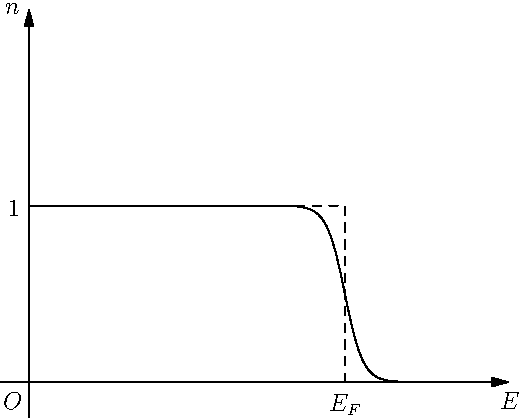
\includegraphics[width=.47\textwidth]{18-Fermi}
\end{figure}

Максимальная энергия электрона при 0К называется энергией Ферми, которая равна
химическому потенциалу при абсолютном нуле температуры:
\[
    E_F = \frac{\hbar^2}{2m}(3\pi^2n)^\frac{2}{3}.
\]
Как видно, при комнатной температуре \( kT \ll E_F \) и лишь небольшая часть
электронов возбуждаются. Таким образом, в процессе нагревания металлов участвует
лишь малая часть всех электронов, что объясняет малую теплоёмкость электронного
газа.
\newpage
